\documentclass[12pt]{article}
\usepackage{mathtools}
\usepackage[papersize={210mm, 270mm},tmargin=17mm,bmargin=15mm,lmargin=15mm,rmargin=15mm]{geometry}
\usepackage[utf8]{inputenc}
\usepackage{graphicx}
\usepackage{fancyhdr}
\pagestyle{fancy}
\lhead[\thepage]{David Cuesta Martín}
\rhead[David Cuesta Martín]{\thepage}
\cfoot{}
\author{David }


\begin{document}
    \textbf{Ejercicio 2: }Como vemos en la siguiente imagen\\
    \begin{center}
        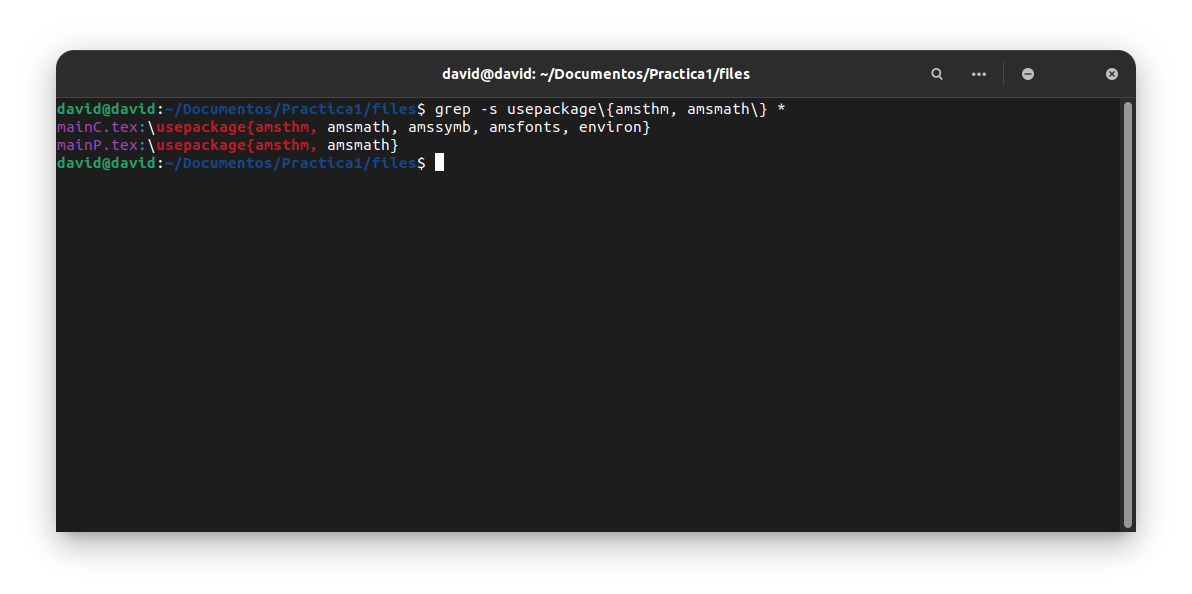
\includegraphics[width=15cm]{img2.png}
    \end{center}
    el comando nos indica que el patron indicado aparece en dos archivos. Realmente el archivo de la linea 2 no es el patron que buscamos, aunque el principio se parezca. El archivo que buscamos es el archivo que nos indican en la línea 3 ya que tenemos el patrón exacto que buscamos.\\ 

    \textbf{Solución: }El archivo buscado es \fbox{\textbf{mainP.tex}}
    
\end{document}
